
\chapter{El sensor Microsoft Kinect}

El sensor Microsoft Kinect \cite{microsoft-kinect}, inicialmente diseñado para la consola de juegos Microsoft Xbox 360 fue lanzado en Noviembre de 2010. Está compuesto por una cámara RGB (rojo, verde, azul), un sensor de profundidad, un conjunto de micrófonos y un mecanismo de inclinación motorizado. \\

\begin{figure}[ht]
\centering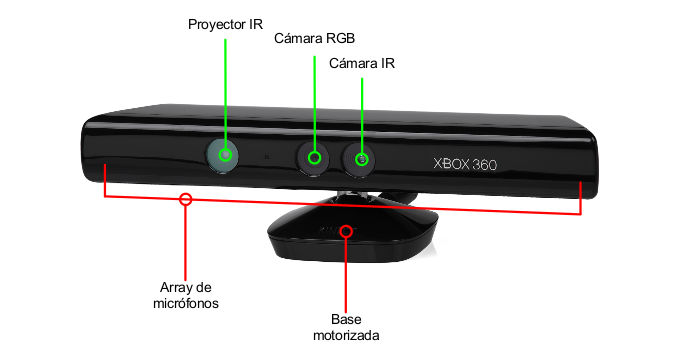
\includegraphics[width=\imsize]
{kinect}
\caption[Microsoft Kinect]
{Microsoft Kinect. Imagen original : Wikipedia bajo licencia Creative Commons\cite{wiki-kinect}.}
\label{fig:kinect}
\end{figure}

\section{Descripción}
\label{sec:descripcion-kinect}
La cámara RGB produce un \textit{stream} de datos de 24 bits por pixel, 8 bits por cada color. Su resolución estándar es 640x480 pixeles con una tasa de muestreo máxima de 30 FPS. \\
El sensor de profundidad está compuesto por un emisor láser infrarrojo (IR) y un sensor CMOS monocromo. Produce un \textit{stream} de datos de 11 bits. Posee una resolución estándar de 640x480 pixeles a una tasa de muestreo máxima de 30 FPS. \\
El campo de visión es de 57° horizontal y 43° vertical. \\
Los cámara presenta otros sensores y un mecanismo de inclinación que no fueron utilizados en este trabajo. \\

Cabe señalar que para un objeto observado en la escena, el valor de profundidad obtenido, no es la distancia real desde la Kinect al objeto, sino la distancia desde el plano del sensor (Figura \ref{fig:esquema-plano-profundidad-kinect}).

\begin{figure}[ht]
\centering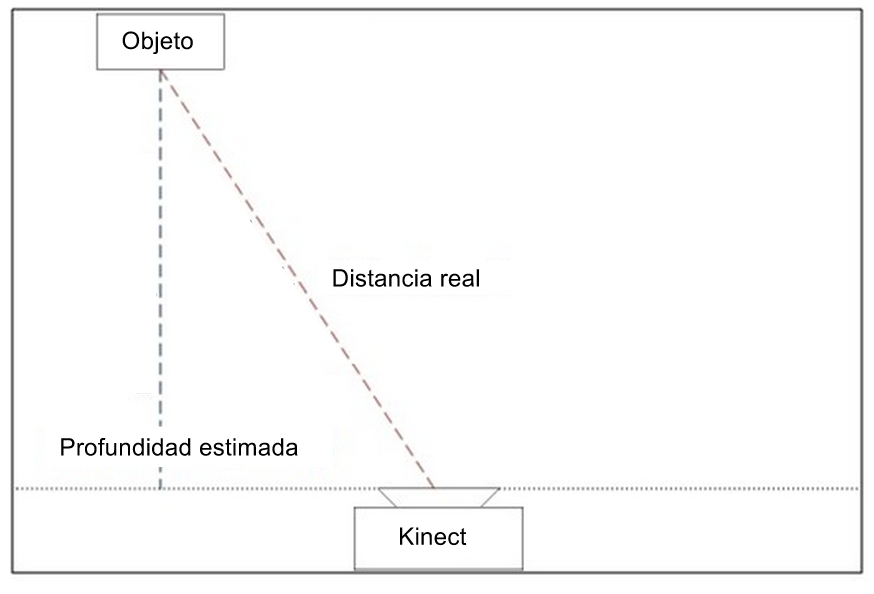
\includegraphics[width=\imsize]
{esquema-plano-profundidad-kinect}
\caption[Esquema de estimación de profundidad Kinect]
{Esquema de estimación de profundidad Kinect. Imagen original \cite{andersen12}.}
\label{fig:esquema-plano-profundidad-kinect}
\end{figure}

\section{Funcionamiento interno}
\label{sec:funcionamiento-kinect}

El funcionamiento de la cámara Kinect esta basado en tecnología propiedad de la empresa israelí PrimeSense \cite{primesense}. \\
Para obtener una imagen de profundidad el emisor láser emite un patrón de puntos que es capturado por la cámara infrarroja (sensor CMOS monocromo). Figura \ref{fig:kinect-patron-ir}. \\

\begin{figure}[ht]
\centering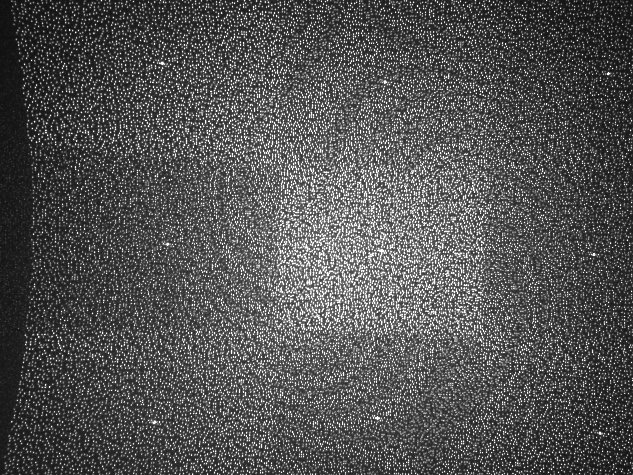
\includegraphics[width=\imsizeS]
{kinect-patron-ir}
\caption[Patrón de puntos emitido por el sensor IR]
{Patrón de puntos emitido por el sensor IR. Fuente : proyecto ROS\cite{ros} bajo licencia Creative Commons.}
\label{fig:kinect-patron-ir}
\end{figure}

El proceso que se describe en la patente de PrimeSense\cite{garcia2008range} se divide en las siguientes etapas :
\begin{enumerate}
\item Capturar el patrón de puntos para un conjunto de imágenes de referencia a diferentes distancias del plano del sensor.
\item Capturar el patrón de puntos sobre una imagen de test de la region de interes.
\item Encontrar la imagen de referencia que mayor similitud tiene con la imagen de test utilizando un método de Correlación Cruzada\cite{wiki-cross-correlation}.
\item Estimar el mapa 3D de la escena por medio de un proceso de triangulación utilizando los desplazamientos entre la imagen de test y la imagen de referencia elegida.
\end{enumerate}

En el caso del Microsoft Kinect, las imágenes de referencia han sido capturadas contra una superficie plana a distancias predefinidas y están almacenadas en el dispositivo. El sensor devuelve la imagen de profundidad en forma de valores de disparidad que luego son traducidos a distancias en metros, en un procedimiento externo, mediante la conversión :

\begin{equation}
distancia=0.1236 \cdot \tan(\frac{disparidad}{2842.5} + 1.1863)
\end{equation}

Si bien el sensor Kinect captura las imágenes RGB y de profundidad de forma independiente, en este trabajo se utiliza una librería que brinda la posibilidad de sincronizar automáticamente ambos tipos de imágenes, dando como resultado una imagen RGB-D o frame RGB-D.

\section{Consideraciones}
\label{sec:consideraciones-kinect}

En este apartado se describen algunas especificaciones para el uso del dispositivo Kinect que se consideran relevantes para este trabajo.

De acuerdo a las especificaciones oficiales, el rango de operación del sensor de profundidad se encuentra entre 0.4 m a 4 m. En Khoshelham\cite{khoshelham2011accuracy} (2011) se analiza la precisión del sensor, midiendo la profundidad de una superficie plana a diferentes distancias y se concluye que el error aleatorio de los datos de profundidad crece cuadráticamente con el aumento de la distancia entre el dispositivo y la escena observada, según se presenta en la figura \ref{fig:error-kinect}.

\begin{figure}[h]
\centering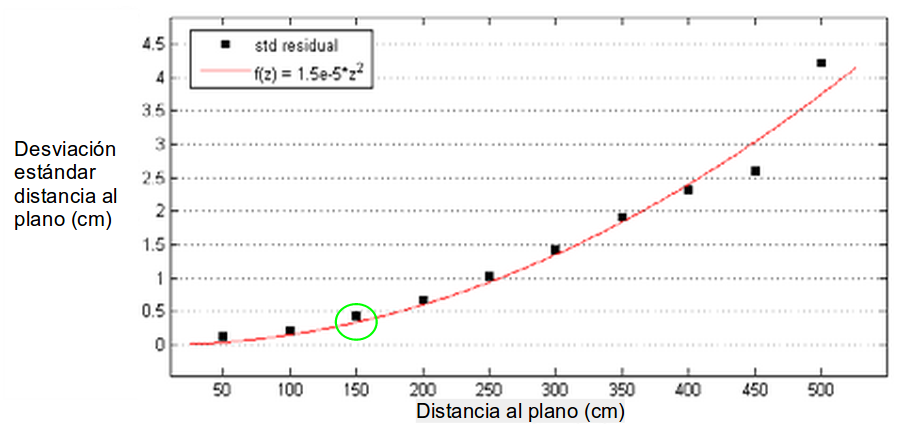
\includegraphics[width=\imsize]
{error-kinect}
\caption[Error camara Kinect]
{Desviación estándar del error en la estimación de profundidad, posicionando el sensor a diferentes distancias del plano de referencia. En rojo se muestra la curva que mejor ajusta al error. La desviación estándar presenta un valor de 0,5 cm a una distancia de 1,5 m y un maximo cercano a 4,25 cm para una distancia de 5 m. Fuente : \cite{khoshelham2011accuracy}.}
\label{fig:error-kinect}
\end{figure}

En Andersen y Ahrendt\cite{andersen12} (2012) se realiza otro análisis del sensor de profundidad del Microsoft Kinect concluyendo lo siguiente :
\begin{itemize}

\item Materiales con características reflectantes influyen sobre el sensor de profundidad imposibilitando la medición de distancias o derivando en mediciones incorrectas.

\item La luz infrarroja, en particular la luz solar, interfiere con el sensor IR limitando su utilización en entornos exteriores.

\item Debido a la distancia interna entre el emisor y el detector IR en el dispositivo Kinect, los objetos iluminados pueden provocar sombras en la imagen de fondo (Figura \ref{fig:sombra-kinect}). La sombra en el patrón imposibilita que el sensor pueda calcular la profundidad y los píxeles en el área sombreada se ponen a profundidad cero. En la figura \ref{fig:silla-sombra-kinect}, se puede observar la imagen RGB (derecha) y de profundidad (izquierda) de una silla. La cámara no pudo capturar la profundidad del borde izquierdo de silla (área en azul) debido a la posición relativa de los sensores IR con respecto a la escena.

\end{itemize}

\begin{figure}[ht]
\centering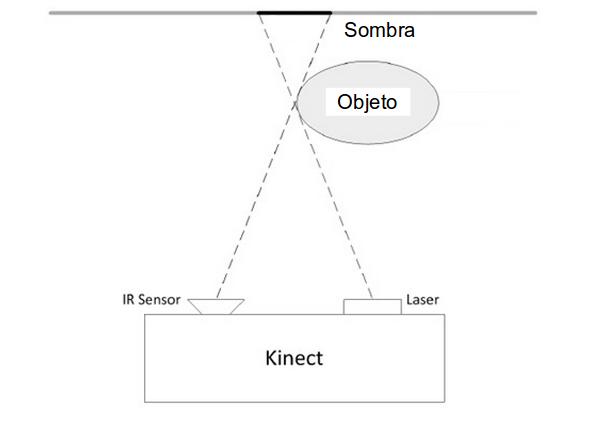
\includegraphics[width=\imsizeS]
{sombra-kinect}
\caption[Esquema de sombras en la imagen de profundidad generada por la cámara Kinect]
{Esquema de sombras en la imagen de profundidad generada por la cámara Kinect. Imagen original : \cite{andersen12}.}
\label{fig:sombra-kinect}
\end{figure}

\begin{figure}[ht]
\centering
\begin{minipage}[h]{.45\textwidth}
\begin{center}
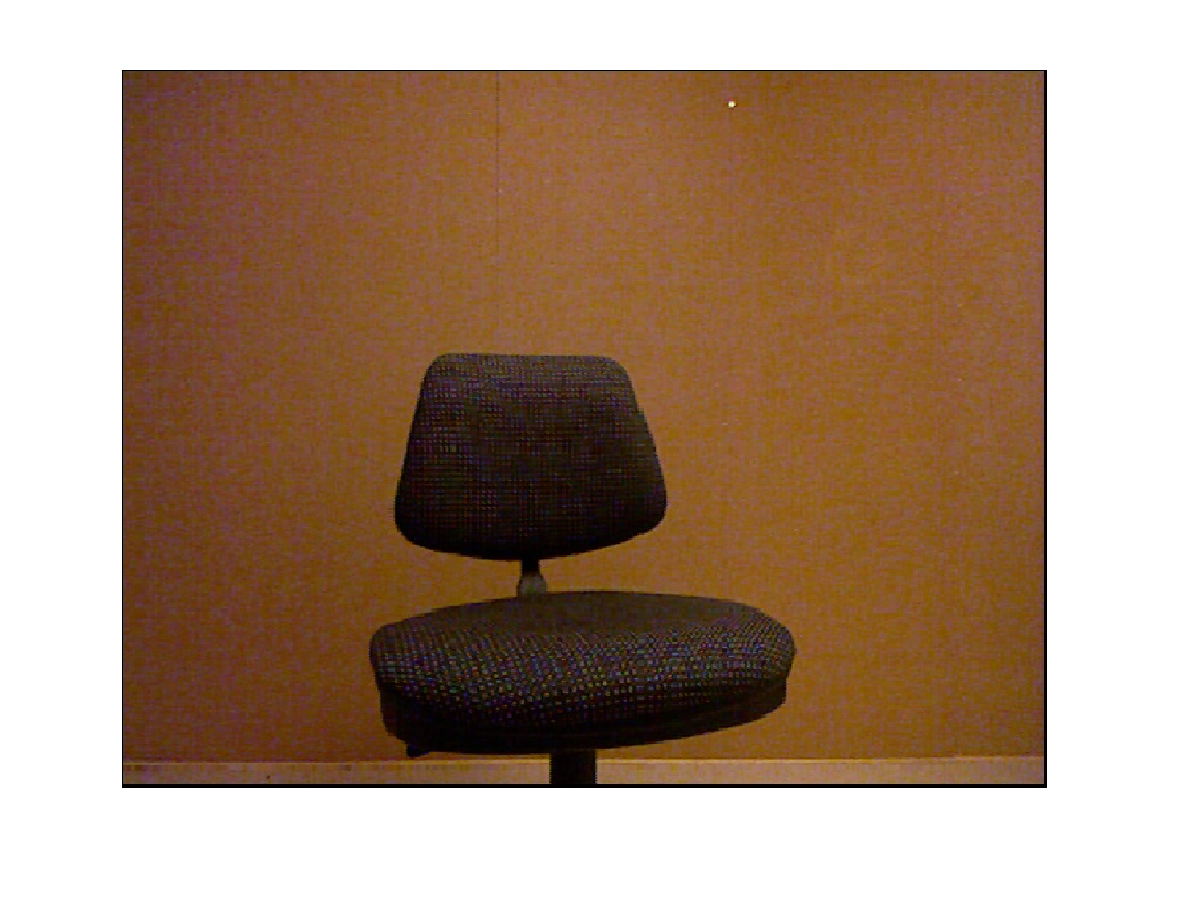
\includegraphics[width=\imsizeS]{silla-rgb-kinect}
\end{center}
\end{minipage}
\hfill
\begin{minipage}[h]{.45\textwidth}
\begin{center}
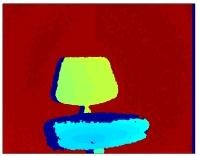
\includegraphics[width=0.91\textwidth]{silla-depth-kinect}
\end{center}
\end{minipage}
\hfill
\caption[Silla con zonas sin medición de profundidad]{Imágenes RGB (derecha) y de profundidad (izquierda) de una silla con zonas sin mediciones de profundidad (en azul). Imagen original : \cite{andersen12}.}
\label{fig:silla-sombra-kinect}
\end{figure}


